%% ============================================================
%%  PŘÍLOHY — Samostatný dokument
%%  Bakalářská práce: Software pro podporu digitalizace
%%                    schvalovacího procesu v malé firmě
%%  Autor: Artem Arsenyev
%%  ČVUT FEL, Katedra počítačů, 2026
%% ============================================================

\documentclass[
  a4paper,
  11pt,
  oneside,
  openany
]{report}

%% ── Kódování a jazyk ─────────────────────────────────────────
\usepackage[T1]{fontenc}
\usepackage[utf8]{inputenc}
\usepackage[czech]{babel}

%% ── Písmo: Latin Modern ──────────────────────────────────────
\usepackage{lmodern}

%% ── Geometrie stránky ────────────────────────────────────────
\usepackage[
  a4paper,
  inner=30mm,
  outer=25mm,
  top=25mm,
  bottom=25mm
]{geometry}

%% ── Barvy ────────────────────────────────────────────────────
\usepackage[dvipsnames]{xcolor}
\definecolor{CTUblue}{HTML}{0065BD}

%% ── Nadpisy ──────────────────────────────────────────────────
\usepackage{titlesec}
\titleformat{\chapter}[block]
  {\normalfont\huge\bfseries\color{CTUblue}}
  {\thechapter}{20pt}{\Huge}
\titleformat{\section}
  {\normalfont\Large\bfseries\color{CTUblue}}
  {\thesection}{1em}{}

%% ── Patičky a hlavičky ───────────────────────────────────────
\usepackage{fancyhdr}
\pagestyle{fancy}
\fancyhf{}
\fancyhead[L]{\textit{Přílohy}}
\fancyhead[R]{\textit{Bakalářská práce}}
\fancyfoot[C]{\thepage}
\renewcommand{\headrulewidth}{0.4pt}

%% ── Obrázky a tabulky ────────────────────────────────────────
\usepackage{graphicx}
\graphicspath{{images/}{images/screenshots/}}

%% ── Listy ────────────────────────────────────────────────────
\usepackage{enumitem}

%% ── Hypertextové odkazy ──────────────────────────────────────
\usepackage[
  colorlinks=true,
  linkcolor=CTUblue,
  citecolor=CTUblue,
  urlcolor=CTUblue,
  pdftitle={Přílohy — Bakalářská práce Artem Arsenyev},
  pdfauthor={Artem Arsenyev}
]{hyperref}
\usepackage{url}

%% ── Informace o práci ────────────────────────────────────────
\newcommand{\ThesisTitle}{Software pro podporu digitalizace schvalovacího procesu v~malé firmě}
\newcommand{\ThesisAuthor}{Artem Arsenyev}
\newcommand{\ThesisSupervisor}{Ing. Martin Dobiáš, Ph.D.}
\newcommand{\ThesisDate}{Květen 2026}

%% ============================================================
\begin{document}

%% ── Titulní strana příloh ────────────────────────────────────
\begin{titlepage}
  \thispagestyle{empty}
  \begin{center}
    \vspace*{1cm}

    
\includegraphics[width=4cm]{LogoCVUT.pdf}\\[1cm]

    {\Large\textbf{České vysoké učení technické v~Praze}}\\[0.3cm]
    {\large Fakulta elektrotechnická}\\[0.1cm]
    {\large Katedra počítačů}\\[3cm]

    {\Huge\bfseries\color{CTUblue}Přílohy k~bakalářské práci}\\[1cm]
    {\large\itshape \ThesisTitle}\\[3cm]

    \begin{flushleft}
      \textbf{Autor:} \ThesisAuthor\\[0.3cm]
      \textbf{Vedoucí práce:} \ThesisSupervisor\\[0.3cm]
      \textbf{Datum:} \ThesisDate
    \end{flushleft}
  \end{center}
\end{titlepage}

\cleardoublepage
\pagenumbering{arabic}
\setcounter{page}{1}

\tableofcontents
\cleardoublepage


%% ============================================================
\chapter{Seznam zkratek a pojmů}
\label{app:zkratky}
%% ============================================================

\begin{description}[leftmargin=3.5cm, style=nextline]
  \item[AS-IS / TO-BE] Současný (AS-IS) a~cílový (TO-BE) stav procesu, terminologie business process management.
  \item[BCrypt] Adaptivní hashovací funkce pro bezpečné ukládání hesel, používá tzv. \emph{salt} a~konfigurovatelný zátěžový faktor.
  \item[BI] Business Intelligence -- analytický nástroj pro reporting a~controlling.
  \item[BPMN] Business Process Model and Notation -- grafický standard pro modelování podnikových procesů.
  \item[CRM] Customer Relationship Management -- systém pro správu vztahů se zákazníky (v~práci INTUO).
  \item[CRUD] Create, Read, Update, Delete -- základní operace nad datovou entitou.
  \item[CSRF] Cross-Site Request Forgery -- útok zneužívající přihlášenou session uživatele.
  \item[DKIM] DomainKeys Identified Mail -- ověření odesílatele e-mailu digitálním podpisem.
  \item[DMARC] Domain-based Message Authentication, Reporting and Conformance -- pravidla pro nakládání s~e-maily, které selžou v~SPF/DKIM.
  \item[DTO] Data Transfer Object -- objekt sloužící k~přenosu dat mezi vrstvami aplikace.
  \item[ERP] Enterprise Resource Planning -- integrovaný informační systém pro řízení podniku.
  \item[GET / POST] Metody protokolu HTTP pro čtení a~zápis dat.
  \item[HTTP / HTTPS] HyperText Transfer Protocol (Secure) -- protokol pro komunikaci v~webu.
  \item[IS] Informační systém.
  \item[JPA] Jakarta Persistence API (dříve Java Persistence API) -- standard pro objektově-relační mapování v~Javě.
  \item[JSON] JavaScript Object Notation -- formát pro výměnu dat.
  \item[L1, L2, L3] Úrovně schvalování ve firmě podle finančních limitů (do~3\,000~Kč, 3\,001--50\,000~Kč, nad~50\,000~Kč).
  \item[MIS] Manažerský informační systém.
  \item[MVC] Model-View-Controller -- architektonický vzor oddělující data, prezentaci a~řízení.
  \item[ORM] Object-Relational Mapping -- překlad mezi objektovým modelem a~relační databází.
  \item[PaaS] Platform as a~Service -- model cloudových služeb (v~práci Railway).
  \item[Pohoda] Účetní a~ekonomický systém využívaný společností Medicton Group.
  \item[RBAC] Role-Based Access Control -- model řízení přístupu na základě rolí.
  \item[REST] Representational State Transfer -- architektonický styl pro webová API.
  \item[Resend] Cloudová služba pro transakční e-mailové notifikace.
  \item[SaaS] Software as a~Service.
  \item[SMTP] Simple Mail Transfer Protocol -- protokol pro doručování e-mailů.
  \item[SPF] Sender Policy Framework -- záznam DNS určující servery oprávněné odesílat e-maily z~domény.
  \item[SQL] Structured Query Language -- jazyk pro práci s~relačními databázemi.
  \item[TLS] Transport Layer Security -- šifrované spojení (dříve SSL).
  \item[UI] User Interface -- uživatelské rozhraní.
  \item[UML] Unified Modeling Language -- standardní jazyk pro modelování softwaru (sekvenční, stavové a~deployment diagramy).
  \item[Workflow] Sekvence kroků zpracování dokumentu nebo požadavku, řízená pravidly a~rolemi.
  \item[XSS] Cross-Site Scripting -- útok vkládáním škodlivého kódu do stránky.
\end{description}


%% ============================================================
\chapter{Obsah přiloženého CD / repozitáře}
\label{app:cd}
%% ============================================================

Zdrojové kódy implementovaného systému, text bakalářské práce a~související
materiály jsou dostupné v~Git repozitáři na adrese
\url{https://github.com/arsenart/Bachelor} (alternativně na přiloženém CD).
Struktura adresáře je následující:

\begin{description}[leftmargin=2.5cm, style=nextline]
\item[\texttt{/Code}] Zdrojový kód aplikace Spring Boot
\item[\quad\texttt{src/main/java/}] Java zdrojové kódy (controllery, služby, entity, repozitáře)
\item[\quad\texttt{src/main/resources/}] Konfigurace, Thymeleaf šablony, lokalizace
\item[\quad\texttt{src/test/java/}] Jednotkové testy (JUnit~5 + Mockito)
\item[\quad\texttt{pom.xml}] Maven konfigurace projektu a~závislosti
\item[\quad\texttt{Dockerfile}] Konfigurace pro kontejnerové nasazení
\item[\quad\texttt{README.md}] Návod ke spuštění a~konfiguraci aplikace
\item[\texttt{/thesis}] Zdrojové soubory bakalářské práce v~\LaTeX{}u
\item[\quad\texttt{main.tex}, \texttt{chapters.tex}] Hlavní soubory práce
\item[\quad\texttt{prilohy.tex}] Tento dokument s~přílohami
\item[\quad\texttt{main.pdf}] Zkompilovaná verze práce ve formátu PDF
\item[\quad\texttt{prilohy.pdf}] Samostatný PDF dokument s~přílohami
\item[\quad\texttt{images/}] Logo ČVUT, BPMN, UML a~architektonické diagramy
\item[\quad\texttt{images/screenshots/}] Snímky obrazovky implementované aplikace
\item[\quad\texttt{zadani.pdf}] Naskenované zadání bakalářské práce
\end{description}

\paragraph{Spuštění aplikace.} Aplikace vyžaduje Javu~17+ a~přístup
k~PostgreSQL~16. Po naklonování repozitáře a~nastavení proměnných
prostředí (\texttt{DB\_URL}, \texttt{DB\_USERNAME}, \texttt{DB\_PASSWORD},
\texttt{RESEND\_API\_KEY}) se aplikace spouští příkazem
\texttt{./mvnw spring-boot:run}. Detailní pokyny jsou v~souboru
\texttt{README.md}.

\paragraph{Online verze.} Funkční nasazení systému je dostupné na adrese
\url{https://bachelor-production-0dda.up.railway.app} v~rámci platformy
Railway s~připojenou produkční databází PostgreSQL.


%% ============================================================
\chapter{Zadání bakalářské práce}
\label{app:zadani}
%% ============================================================

Originál zadání bakalářské práce podepsaný děkanem fakulty a~vedoucím
katedry je vložen na následujících stranách jako naskenovaný PDF dokument.

\IfFileExists{zadani.pdf}{%
  \cleardoublepage
  \thispagestyle{empty}
  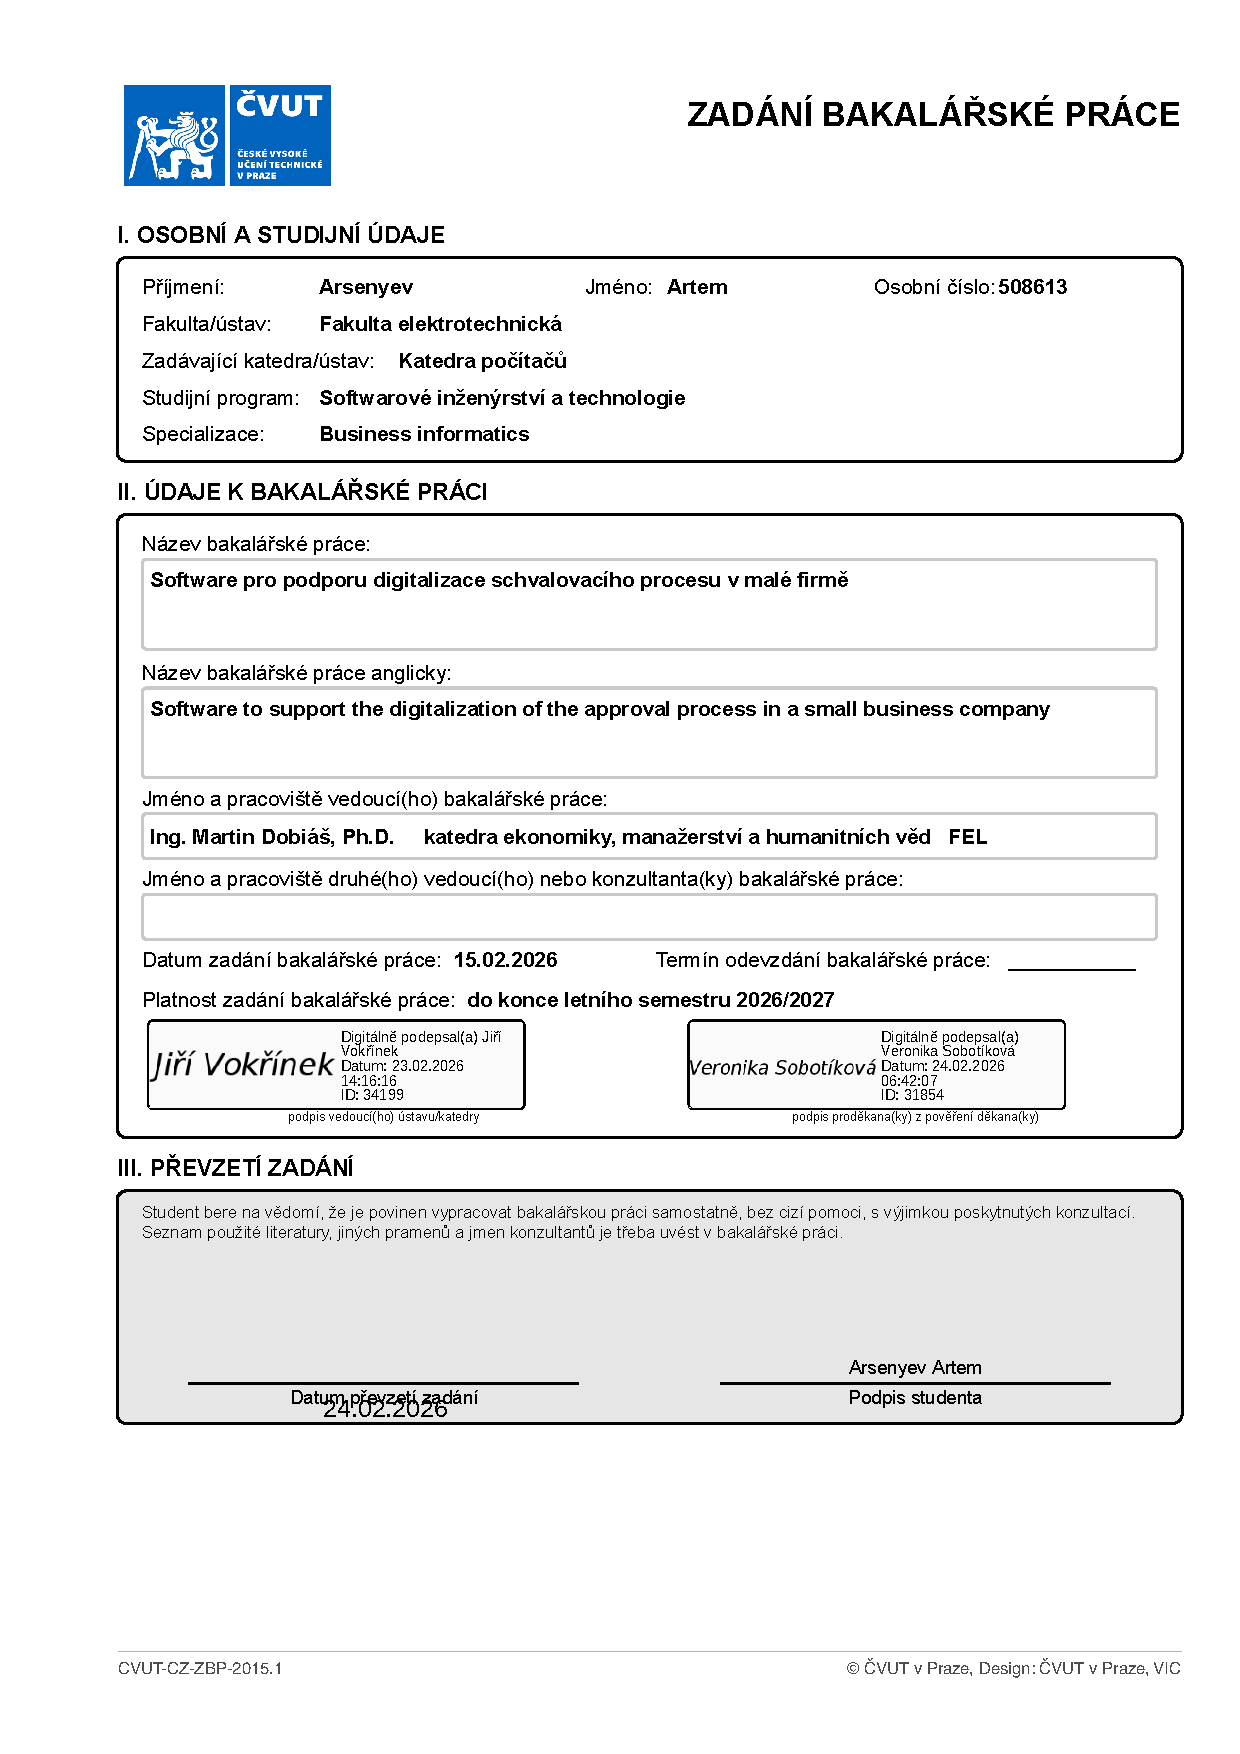
\includegraphics[width=\textwidth,page=1]{zadani.pdf}
  \cleardoublepage
  \thispagestyle{empty}
  \includegraphics[width=\textwidth,page=2]{zadani.pdf}
}{%
  \textit{(Soubor zadani.pdf nebyl nalezen.)}
}


\end{document}
